\setchapterpreamble[u]{\margintoc}
\chapter{物理中的代数与几何}
\labch{intro}


\section*{章节导论:对称性与对称性破缺}
仍在画饼,可以参考这篇知乎文章,写的很不错:\href{https://zhuanlan.zhihu.com/p/338221764}{知乎专栏}

在前言中,我们提到过实际非高能物理方向是完全不需要太多数学的,但是就实际过程中,常常有人问我这些需不需要学,需不需要看,既然如此,那么干脆直接全部学一遍.不过为了篇幅考虑,大部分定理不会去证明,只不过是粗浅的讨论一遍这些内容而已.\\
\textbf{这部分只不过是对绝大部分的可能应用的数学内容的概括,可以直接从第二章开始看!}

需要强调的是,受限于章节内容,我们的出发角度都是物理角度,且较为狭隘和数学上有\textbf{很大区别},想深入了解可以参考一些经典案例:
\begin{enumerate}
    \item 微分流形:流形导论(Loring W.Tu)
    \item 李代数:Lie Groups,Lie Algebras,and Representations:An Elementary Introduction(Brian C. Hall)
    \item 辛几何:经典力学的数学方法(阿诺尔德);Lectures on Symplectic Geometry(da Silva)
\end{enumerate}

\section{李群(Lie Group)初步}
\subsection{群与李群(Lie Group)}
我们或许听说过一个说法:``物理学的关键是对称和守恒",而诺特定理给出了对称性与守恒性的联系,例如,时间平移不变性意味着能量守恒;空间平移不变性意味着动量守恒;转动不变性意味着角动量守恒;电势和向量势的规范不变性得出电荷的守恒等.而描述对称性的语言就是群论.


我们可以认为群是一类拥有特殊结构的集合,即满足如下关系的集合\sidenote[][]{当然,这里会忽略对于主线无用的那些群论内容,所以如果和数学系的抽象代数对比,你甚至可能会感觉到学的不是同一个东西}:
\marginnote[]{这一章虽然名字比较吓人,但并没有太过深入讲解李群与李代数,主要为了帮助物理系学生来快速对这一门学科建立印象.当然,我们不能保证在后续的不断更新中是否会改变这一点,在最初的版本中,这一章被置于第三章,也就是初量的后续部分,以及这一章的进度只会跟进后续章节的需要,也就是说这一章的全部已完成内容足以支撑起后续章节的学习.}
\textbox{群的定义}{
    设$G$是一个集合,若满足下面4个条件,则称$G$为一个群(Group)
    \tenum{\item $G$中存在一种运算规则,对$G$中的任意两个元素$g,h\in G$,存在对应$G$中的一个元素,记为
        \begin{equation}
            k=g\circ h(k=gh)
        \end{equation}
        \item 运算规则满足交换律,对$G$中的任意三个元素$g,h,k\in G$,存在
        \begin{equation}
            (gh)k=g(hk)
        \end{equation}
        \item $G$中存在一个幺元$e$(有时也称单位元),使得对于$G$中任意元素$g$,均有
        \begin{equation}
            ge=eg=g
        \end{equation}
        \item $G$中每一个元素$g$,均存在一逆元$g^{-1}$,使得
        \begin{equation}
            gg^{-1}=g^{-1}g=e
        \end{equation}
    } }
我们可以发现,群的运算规则通常不满足交换律,特殊的,我们把满足交换律的群称为阿贝尔群(Abel Group)\sidenote[][]{关于这个有一个经典笑话:一位美国数学教授来到法国,见路边有一小孩,遂上前问到:“小朋友,你知道1+2等于几吗?”小孩摇摇头说:“不知道.”教授正想感叹法国数学教育如此之落后,却听到小孩接着说:“虽然我不知道1+2等于几,但是我知道1+2等于2+1,因为整数加法群是阿贝尔群!”}.
\textbox{子群的定义}{设$G$是一个群,$H$为$G$的一个子集($H\subseteq G$),若$H$按照$G$的运算规则仍是一个群,则称$H$是$G$的子群.}
下面我们将给出一系列典型的群的实例,请根据定义思考它们是怎么构成的,并且尝试找到一些共性.
\marginnote[]{\ref{enum:1}都不是,首先对于无理数我们注意到$\pi+(-\pi)=0$,而0不是无理数,故无理数不构成加法群.同样的,我们注意到$1+(-1)=0$,0同样也不是奇数,故奇数也不构成加法群.\\ \ref{enum:2} 答案是显然的,群中幺元为1,但$0/0$无意义.}
\ytextbox{例子}{
    \ytenum{
        \item 全体实数$\mathbb{R}$(或复数$\mathbb{C}$),对加法构成一个阿贝尔群.\\
        我们知道有理数全体是$\mathbb{R}$的子群,而全体偶数是有理数的子群,自然也是$\mathbb{R}$的子群,那么存在一个问题:无理数全体,或奇数全体是否是$\mathbb{R}$的子群?\label{enum:1}
        \item 全体实数除去零$\mathbb{R}/0$或全体复数除去零$\mathbb{C}/0$对乘法构成阿贝尔群.\\
        同样的,我们有个问题:为什么要除去0?\label{enum:2}
        \item $G =\{1,-1,i,-i\}$对复数乘法运算构成一有限阿贝尔群.这里1是$G$的幺元,而-1的逆元就是-1,$i$与$-i$互为逆元.
        \item 行列式不为零的n阶实矩阵全体对矩阵乘法构成一个群,$n$阶全线性群,其记为$GL(n,R)$,它的元素由$n^2$个独立实参数所确定.其是一个$n^2$维(不可交换)李群,在后面我们会再次讨论它.
        \item 行列式为 1 的 2 阶实矩阵全体对矩阵乘法构成一个群:二阶(实)特殊线性群$SL(2,R)$.因为二阶实矩阵$\begin{bmatrix}a&b\\c&d\end{bmatrix}$由四个实数$a,b,c,d$ 构成,由于行列式为1的要求,使他们必须满足条件:$ad-bc=1$.所以$SL(2,R)$ 中的元素由3个独立的实参数所确定.按照下面将要给出的定义可见$SL(2,R)$ 是一个三维(不可交换)李群,而且它是$GL(2,R)$的子群.
        \item 行列式为 1 的 n 阶实矩阵全体对矩阵乘法构成一个群:n阶特殊线性群$SL(n,R)$,这是一个$n^2-1$维(不可交换)李群,而且它是$GL(n,R)$的子群.
        \item 行列式不为0的 n 阶复矩阵全体对矩阵乘法构成一个群:n阶(复)全线性群$GL(n,C)$,行列式为 1 的 n 阶复矩阵全体对矩阵乘法构成一个群:n阶(复)特殊线性群$SL(n,C)$.\\
        $GL(n,C)$是一个$2n^2$维(不可交换)李群,$SL(n,C)$是一个$2n^2-12$维(不可交换)李群.
    }
    }

我们发现,所举的例子(除第一个外)都存在共同点:元素都是矩阵(实数和复数可看作一阶矩阵),群的运算法则都是矩阵乘法.我们把这类群统称为\textbf{线性群},线性群也是最具代表性的一类李群,今后所使用的李群基本上都是线性群.
\marginnote[]{事实上,从现在开始,我们就已经走上物理的道路上了,实际上,哪怕你掌握了这一章的全部内容,可能对于数学上的抽象代数那一套仍非常陌生,但早已足够应付物理上的内容了.在上一段,我们给出了一个断言:``今后所使用的李群基本上都是线性群",实际上,我们完全可以这么说,如果不去碰高能和那些fancy的理论(例如弦论,Ads/CFT等),哪怕仅掌握$U(1),SU(2),SU(4)$,$SO(2),SO(3)$这几个群和其表示论对于凝聚态学习就远远足够了.}

下面我们正式进入李群这一部分的内容.
\textbox{Lie群的定义}{\label{def:1.3}
设$G$是一个$r$维流形,同时$G$又是一个群,并将其幺元记为$e$,因$e$又是流形$G$中的一点,所以可取定一个包含$e$的局部坐标邻域$U$;在$U$中取定坐标系$\{U,\varphi\}$.设取$e$为坐标原点,有
\begin{equation}
    \varphi(e)=(0,0,\cdots,0)
\end{equation}
任取$U$中的三个元素$g,h,k$,并设其坐标为
\begin{equation}
    \begin{aligned}
        \varphi(g)&=(x_1,x_2,\cdots,x_r)\\
        \varphi(h)&=(y_1,y_2,\cdots,y_r)\\
        \varphi(k)&=(z_1,z_2,\cdots,z_r)
    \end{aligned}
\end{equation}
而群乘法$k=gh$则可以被定义为以下形式:
\begin{equation}
    \begin{aligned}
        &z_{1}=f_{1}(x_{1},\cdots,x_{r};y_{1},\cdots,y_{r})\\
        &z_{2}=f_{2}(x_{1},\cdots,x_{r};y_{1},\cdots,y_{r})\\
        &z_{r} =f_r(x_1,\cdots,x_r;y_1,\cdots,y_r) 
    \end{aligned}
\end{equation}
我们要求这$r$个函数$f_1,f_2,\cdots,f_r$是无限次可导的(光滑的).我们把这$r$个函数$f_1,f_2,\cdots,f_r$称为$G$的\textbf{乘法函数}.其完全确定了群$G$的结构.我们把这样的群$G$叫做一个$r$维李群.
}
我们现在根据群的定义来给出几个自然性质
\begin{enumerate}
    \item 第一个定义是显然的,因为李群的定义建立在这种运算规则上,我们只需要对另外3个条件进行讨论.
    \item 我们现在给出交换律所导出的性质,为方便表述,我们简记群乘法关系为$z=f(x,y)$:
    \begin{equation}
        f(f(x,y),z)=f(x,f(y,z))
    \end{equation}
    \item 对于幺元$e$,其坐标为$(0,0,\cdots,0)$,所以有$ex=xe=x$.
    \begin{equation}
        f(x,0)=f(0,x)=x
    \end{equation}
    \item 对于逆元$g^{-1}$,我们设其坐标为$(\tilde{x}_1,\cdots\tilde{x}_r)$,于是有
    \begin{equation}
        f(x,\tilde{x})=f(\tilde{x},x)=0
    \end{equation}
\end{enumerate}
我们很容易看出,乘法函数是很抽象的,只有乘法函数来研究李群往往是无处下手的(更何况我们是学物理的),于是有了李代数的理论.不过在展开李代数之前,我们使用几个实际的李群的例子来帮助建立对于李群的理解.
\textbox{实例(1)}{
    $T_2=\Big\{\begin{bmatrix}e^{x_1}&x_2\\0&1\end{bmatrix}\Big|x_1,x_2\in\mathbb{R}\Big\}$.这个群的元素由两个独立实参数$x_1,x_2$决定.所以,$T_2$是一个二维流形,我们现在来逐个验证其满足群的要求.
\begin{proof}
    依次逐条验证性质:
    \tenum{
        \item 首先我们验证其封闭性
        \begin{equation}
            \begin{gathered}\begin{bmatrix}e^{x_1}&x_2\\0&1\end{bmatrix}\begin{bmatrix}e^{y_1}&y_2\\0&1\end{bmatrix}=\begin{bmatrix}e^{x_1}e^{y_1}&e^{x_1}y_2+x_2\\0&1\end{bmatrix}\\=\begin{bmatrix}e^{x_1+y_1}&e^{x_1}y_2+x_2\\0&1\end{bmatrix}=\begin{bmatrix}e^{z_1}&z_2\\0&1\end{bmatrix}\in T_2\end{gathered}
        \end{equation}
        并同时写出其乘法函数,不难发现其乘法函数是无限次可微的.
        \begin{equation}
            \begin{aligned}&z_{1}=f_{1}(x_{1},x_{2};y_{1},y_{2})=x_{1}+y_{1},\\&z_{2}=f_{2}(x_{1},x_{2};y_{1},y_{2})=e^{x_{1}}y_{2}+x_{2}.\end{aligned}
        \end{equation}
        \item $T_2$的乘法运算为矩阵乘法,自然满足结合律.
        \item 对于幺元,我们注意到
        \begin{equation}
            \begin{bmatrix}e^0&0\\0&1\end{bmatrix}=\begin{bmatrix}1&0\\0&1\end{bmatrix}
        \end{equation}
        \item 我们注意到有
        \begin{equation}
            \begin{aligned}\begin{bmatrix}e^{-x_1}&-x_2e^{-x_1}\\0&1\end{bmatrix}\begin{bmatrix}e^{x_1}&x_2\\0&1\end{bmatrix}&=\begin{bmatrix}e^{x_1}&x_2\\0&1\end{bmatrix}\begin{bmatrix}e^{-x_1}&-x_2e^{-x_1}\\0&1\end{bmatrix}\\&=\begin{bmatrix}1&0\\0&1\end{bmatrix}\end{aligned}
        \end{equation}
        所以逆元为$\begin{bmatrix}e^{-x_1}&-x_2e^{-x_1}\\0&1\end{bmatrix}$并容易验证其不满足交换律.
        }
\end{proof}}
\textbox{实例(2)}{    我们的下一个实例是绕定轴转动的旋转群SO(2),显然,我们只需要一个变量(转动角$\theta$)就可以表述一个转动变换,所以我们表示群元为$g(\theta)$,其中$\theta$的取值范围是$[0,2\pi)$.而群的运算法则可以被规定为相继的两个转动,即转动角相加,但需要保持转动角始终在取值范围内.我们可以使用公式表达:
    \begin{equation}
        g(\theta_1)g(\theta_2)=g(\theta_{12}),\qquad\theta_{12}=(\theta_1+\theta_2)\mod 2\pi
    \end{equation}
    我们容易验证其满足对应的4条性质.不过我们在关于线性代数的学习中,我们知道:我们也可以使用旋转矩阵来表述定轴转动.
    \begin{equation}
        \begin{bmatrix}x\\y\end{bmatrix}\xrightarrow{g(\theta)}\begin{bmatrix}x'\\y'\end{bmatrix}=\begin{bmatrix}\cos\theta&-\sin\theta\\\sin\theta&\cos\theta\end{bmatrix}\begin{bmatrix}x\\y\end{bmatrix}=\begin{bmatrix}x\cos\theta-y\sin\theta\\x\sin\theta+y\cos\theta\end{bmatrix}
    \end{equation}
    我们发现,旋转矩阵是SO(2)群的群元.我们在下一个例子会更加深入讨论这部分内容.}
    \begin{marginfigure}
        \centering
        \includegraphics[width=0.4\linewidth]{"images/Euler angle"}
        \caption{欧拉角}
        \label{fig:euler-angle}
    \end{marginfigure}
    \textbox{实例(3)}{
    现在我们需要讨论三维旋转群SO(3),其群元表示三维空间中绕某个固定点的一个转动$g\in SO(3)$,为了方便表述SO(3),我们使用如图所示的欧拉(Euler)角$(\alpha,\beta,\gamma)$来表示一个转动.
    
    \marginnote[*6]{我们依次写出绕$z$轴旋转$\alpha$角;绕$x$轴旋转$\beta$角;绕$z$轴旋转$\gamma$角的三个群元的矩阵表示:
        $$g_z^\alpha={\begin{bmatrix}\cos \alpha &-\sin \alpha &0\\\sin \alpha &\cos \alpha &0\\0&0&1\end{bmatrix}}$$
        $$g_x^\beta={\begin{bmatrix}1&0&0\\0&\cos \beta &-\sin \beta \\0&\sin \beta &\cos \beta \end{bmatrix}}$$
        $$g_z^\gamma={\begin{bmatrix}\cos \gamma &-\sin \gamma &0\\\sin \gamma &\cos \gamma &0\\0&0&1\end{bmatrix}}$$
    }
    
    我们给出最终群元的表示:
    \begin{equation}
        g=g_z^\alpha g_x^\beta g_z^\gamma
    \end{equation}
    因此,SO(3)的元素可以通过三个独立参量$\alpha,\beta,\gamma$来确定,因此不难验证SO(3)是一个三维李群.
    
    现在我们给出另一种表述SO(3)的方法.\\
    我们对于两个矢量$x=(x_1,x_2,x_3),y=(y_1,y_2,y_3)$给出三维欧式空间$\mathbb{R}_3$的内积:
    \begin{equation}
        \langle x,y\rangle=\sum_{j=1}^{3}x_j y_j=x_1y_1+x_2y_2+x_3y_3
    \end{equation}
    我们定义一个线性变换算符$g=(g_{ij})$,存在关系
    \begin{equation}
        \begin{aligned}
            x\xrightarrow{g}x'=gx=\begin{bmatrix}g_{11}&g_{12}&g_{13}\\g_{21}&g_{22}&g_{23}\\g_{31}&g_{32}&g_{33}\end{bmatrix}\begin{bmatrix}x_1\\x_2\\x_3\end{bmatrix}\\ g\in SO(3)\Leftrightarrow\langle gs,gy\rangle=\langle x,y\rangle\quad\forall x,y\in\mathbb{R}_3\quad\text{且}\det g>0
        \end{aligned}
    \end{equation}
    而且我们发现$\langle gs,gy\rangle=\langle x,g^Tgy\rangle$,其中$g^T$表示$g$的转置,即$g_{ij}^T=g_{ij}$,我们根据刚才所给出的关系发现$\langle x,g^Tgy\rangle=\langle x,y\rangle$,即$g^Tg=\textbf{1}$,我们把满足关系$g^Tg=gg^T$的线性变换构成的群称为正交群.
    
    对于3阶矩阵$g$,存在9个元素,但为了满足特殊正交群的特殊性($\det g=1$)和正交性($g^Tg=gg^T$),共有6个方程需要满足.所以,我们可以拿出3个作为独立参数,这再次证明了$g$可以表述SO(3)这个三维李群.
    }

    
\subsection{指数映射与对数映射}
\marginnote[]{在前面的部分,我们强调了群的乘法一般不可交换,这直接导致了刻画李群的乘法函数变得非常复杂,这意味着想通过研究乘法函数来研究李群是不现实的.而为了研究李群的各种结构,我们可以对李群在幺元处的无穷小变换进行研究,而Lie证明了李群的主要特征可以通过无穷小变换来得到,这就是为什么现在称这类群为李群的原因.}对于无穷小变换,它是一个拥有特殊结构的线性空间,我们称它构成的代数结构为\textbf{李代数}.

这里,我们再次强调,后面默认所有的群都是\textbf{线性群},群的运算规则都是\textbf{矩阵乘法}!

我们回到这一节前面所提到的,由于矩阵乘法不可交换,导致运算变得复杂,那么有没有一种办法,可以让复杂的运算变为较简单的运算呢(最好还是物理中最喜欢的线性运算)?

答案是肯定的,我们高中就学过一种特殊的运算:指数运算,它可以把较为复杂的乘法变为较为简单的加法,即对于给出的$y_1=e^{x_1},y_2=e^{x_2}$,我们有
\begin{equation}
    y_1y_2=e^{x_1}e^{x_2}=e^{x_1+x_2}
\end{equation}
这样,我们就实现了运算的``降级",并且还是线性运算.现在,问题变为,我们能否同样应用这种方式,将矩阵乘法转变为某种加法呢?

答案同样是肯定的,但由于矩阵乘法比代数乘法更为复杂,相应的``加法"自然也更加复杂.而为了得到这种简单的``加法"运算,我们首先对$n$阶矩阵$A$定义幂指数:
\begin{equation}
    e^A=\exp(x)=\textbf{1}+A+\frac{A^2}{2!}+\frac{A^3}{3!}+\cdots 
\end{equation}
易证此级数对于任意的矩阵$A$都是收敛的.并且对于零矩阵$O$,显然有
\begin{equation}
    e^O=\textbf{1}
\end{equation}
并且,前面我们多次提到矩阵乘法相比代数乘法是不可交换的,那么,反应到对应的``加法"运算上,自然也有区分加法的性质,即当且仅当$A,B$对易的时候,才有$e^Ae^B=e^{A+B}$,这是主要的困难点,那么我们的主要问题就集中在$e^Ae^B=e^{?}$上,这也就是我们将要学习的李代数的内容.不过,在正式开始李代数的内容之前,我们先讨论一下其他同样有价值的内容.

我们仅了解了和指数函数对应的运算,而我们高中还知道,指数函数的逆运算是对数函数,接下来我们效仿之前的内容,对对数函数应用同样的定义方法:

同样对于$n$阶矩阵$A$,我们定义\sidenote[][]{在物理的语境中,$\log$通常仅指$\ln$,同样的,本文中采取该写法.}
\begin{equation}
    \log A=(A-\textbf{1})-\frac{(A-\textbf{1})^2}2+\frac{(A-\textbf{1})^3}3-\frac{(A-\textbf{1})^4}4+\cdots 
\end{equation}
不同于指数函数,为了保证级数收敛,我们要求$A-\textbf{1}$的每一个元素的绝对值均小于$\dfrac{1}{n}$,即要求$A$是与幺元邻近的元素.并且指数函数与对数函数互为逆运算的关系对于这个定义同样适用(仅需泰勒展开即可证明,留给读者自行尝试).
\subsection{单参数子群}
在前面,我们通过代数方法初步建立了一些对应关系,这一小节,我们通过几何的角度再次考虑这个对应关系.
\textbox{单参数子群}{设$G$为一个李群,并且$\gamma(t)(-\infty<t<\infty)$为$g$中过幺元$e$的一条曲线,则对每一取定的$t_0\in \mathbb{R},\gamma(t_0)$是$G$中的一个元素.并设参数$t$满足:
    \begin{equation}
        \gamma(t_1+t_2)=\gamma(t_1)\gamma(t_2)
    \end{equation}
    则称$\gamma(t)$是$G$中的一个单参数李群.}

现在我们通过几何的角度思考问题.

我们将李群$G$的一个单参数子群看成流形$G$ (对二维Lie 群,可将$G$ 看成为一张曲面)中过$e$处的一条曲线.从微积分知道这只要对$\gamma\left(t\right)$在$t=0$处求导即得$\gamma\left(t\right)$在$t=0$处的切向量,$\gamma^\prime(0)=\frac{\d\gamma(t)}{\d t}$.(因为我们只讨论线性群,所以$\gamma\left(t\right)$是矩阵,其元素是$t$ 的函数,$\gamma^{\prime}(t)$ 表示对$\gamma(t)$的每一元素求导所得的矩阵).由于:
\begin{equation}
    \gamma (t+s)=\gamma (t)\gamma (s)
\end{equation}
两边对$s$求导,同时令$s=0$,得到一个微分方程
\begin{equation}
    \gamma' (t)=\gamma(t)\gamma' (0)
\end{equation}
对于这类微分方程,我们知道其解为
\begin{equation}
    \gamma(t)=\exp(t\gamma'(0))
\end{equation}
由此,我们知道,单参数子群必能表达为指数映射的形式.\\
\begin{marginfigure}
    \centering
    \caption{二维李群与其单参数子群}
    
    
    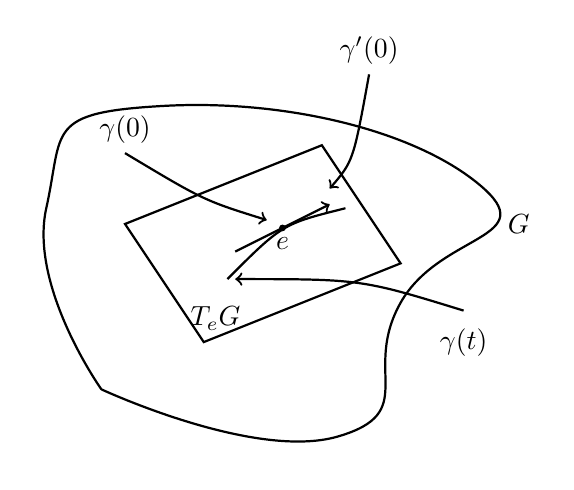
\begin{tikzpicture}
        
        % Draw the manifold G
        \draw[thick] plot [smooth,tension=1] 
        coordinates {(0.2,1.4) (3.2,0.8) (4,2.5) (5,4) (1,5) (-0.5,3.7) (0.2,1.4)};
        %\draw[thick] (0,0) to[out=30, in=180] (4,2.5) to[out=0, in=270] (5,4) to[out=90, in=30] (1,5) to[out=210, in=150] cycle;
        
        % Label G
        \node at (5.5,3.5) {$G$};
        
        % Draw the tangent space T_eG
        \draw[thick] (1.5, 2) -- (4, 3) -- (3, 4.5) -- (0.5, 3.5) -- cycle;
        
        % Label TeG
        \node at (1.65, 2.3) {$T_e G$};
        
        % Draw the curve \gamma(t)
        \draw[thick] (1.8, 2.8) .. controls (2.5, 3.5) .. (3.3, 3.7);
        
        % Label points and vectors
        \node at (0.5,4.7) {$\gamma(0)$};
        \draw[thick, ->] (0.5,4.4) .. controls (1.5,3.8) .. (2.3,3.55);
        \node at (4.8, 2) {$\gamma(t)$};
        \draw[thick, ->] (4.8,2.4) .. controls (3.5,2.8) .. (1.9,2.8);
        \filldraw[black] (2.5,3.45) circle (1pt) node[anchor=north] {$e$};
        \draw[thick, ->] (1.9, 3.15) -- (3.1, 3.75);
        \node at (3.6, 5.7) {$\gamma'(0)$};
        \draw[thick, ->] (3.6, 5.4) .. controls (3.4,4.3) .. (3.1,3.95);
        
    \end{tikzpicture}
\end{marginfigure}
由解的形式可见,对于$G$在幺元处的切空间$T_eG$的任意一个向量$A=\gamma'(0)$,就有$G$中的一元素$\gamma(1)=\exp(\gamma'(0))$与之对应.现在我们稍微总结一下:对于李群$G$这个流形,我们可以找到其单参数子群$T_eG$作为其切空间,并且我们可以找到一个指数映射从切空间到原空间,很快,当我们学会李代数的时候,我们会再次使用李代数的语言来总结:``李代数就是李群的切空间所导出的代数".

我们再次回到群$G$和它的单参数子群,我们发现,如果给定$G$中与幺元邻近的一个元素\sidenote[][]{当然,由于我们研究线性群,幺元为单位矩阵.}$g$,并定义向量$A=\log g$,则由$e^A=g$ 知,$A$ 为$G$ 在$e$ 处之切向量,$e^tA$为以 $A$ 为单位切向量的单参数子群.因此,对$G$ 中与幺元$e$ 邻近的一个元素就有$T_{e}(G)$($G$ 在幺元处的切空间)中一向量$A$ 与之对应,也就是说,设$U\subset G$ 中包含$e$ 的一个适当邻域,我们建立了一种对应关系
\begin{equation}
    \begin{aligned}
        G\supset U&\overunderset{\log}{\exp}{\longleftrightarrow}T_{e}(G)\\g&\to A=\log g\\e^{A}&\leftarrow A
    \end{aligned}
\end{equation}
这种对应关系可以使我们对李群的研究转化到与其对应的在幺元$e$处的切空间$T_e(G)$.而我们知道,$T_e(G)$是由向量组成的线性空间,其线性结构具有先天优势,拥有远比李群简单的结构和运算.但由于我们前面所提到的,由于矩阵乘法相比于数乘的不可交互性,自然由此导出的切空间的运算自然也不能简单用普通加减法来表述,即右侧关系图
\marginnote[]{$$\begin{aligned}&T_{e}(G)\qquad G\\&A\quad\longrightarrow\quad e^{A}\\&B\quad\longrightarrow\quad e^{B}\\&A+B\to e^{A+B}\ne e^{A}e^{B}\end{aligned}$$}

为此,我们迫切需要引入一种新的代数结构来反映$G$中的不可交换性,而具有这种新结构的线性空间$T_e(G)$
,就是我们下一节所要讲的\textbf{李代数}.
\section{李群与李代数}
\subsection{李代数}
由上面的讨论,我们现在知道$e^Ae^B\ne e^{A+B}$,那么,问题自然变为:$e^Ae^B=e^{?}$,或者表述为,$G$的单参数子群的代数结构是什么样的?

为了解决这个问题,我们设$A,B\in T_e(G)$,取一个参数$t$,并要求$|t|$适当小,从而能够保证$e^{tA}$与$e^{tB}$均为李群$G$中与幺元$e$邻近的元素\sidenote[][]{这个要求是必要的,我们需要满足后续使用级数的收敛性.}.现在我们构造一个函数:
\begin{equation}
    g(t)=e^{tA}e^{tB}e^{-tA}e^{-tB}
\end{equation}
显然,对于特例,即如果$e^{tA}$与$e^{tB}$可交换,$g(t)=e=\textbf{1}$,对于不可交换的情况,$g(t)$与幺元$e$的偏离程度反映了$e^{tA}$与$e^{tB}$的乘法与可交换的乘法之间的差异大小.现在我们具体分析$g(t)$.
\marginnote[]{展开的计算过程
$$\begin{aligned}
    g(t)& =e^{tA}e^{tB}e^{-tA}e^{-tB} \\
    &=(\textbf{1}+tA+\frac{t^{2}}{2!}A^{2}+\frac{t^{3}}{3!}A^{3}+\cdots)\\&\quad\times(\textbf{1}+tB+\frac{t^{2}}{2!}B^{2}+\frac{t^{3}}{3!}B^{3}+\cdots) \\&\quad\times(\textbf{1}-tA+\frac{t^2}{2!}A^2-\frac{t^3}{3!}A^3+\cdots)\\&\quad\times(\textbf{1}-tB+\frac{t^2}{2!}B^2-\frac{t^3}{3!}B^3+\cdots) \\
    &=\{\textbf{1}+t(A+B)+t^{2}(\frac{A^{2}}{2}+AB+\frac{B^{2}}{2})\\&\quad+t^{3}(\frac{A^{3}}{6}+\frac{A^{2}B}{2}+\frac{AB^{2}}{2}+\frac{B^{3}}{6})+O(t^{4})\} \\
    &\quad\{\textbf{1}-t(A+B)+t^2(\frac{A^2}{2}+AB+\frac{B^2}{2})\\&\quad-t^3(\frac{A^3}{6}+\frac{A^2B}{2}+\frac{AB^2}{2}+\frac{B^3}{6})+O(t^4)\} \\
    &=\textbf{1}+t(A+B-A-B)+t^{2}(AB-BA)+\\&\quad t^{3}(\frac{A^{2}B}{2}-\frac{AB^{2}}{2} \\
    &\quad-\frac{B^2A}{2}+\frac{BA^2}{2}-ABA+BAB)+O(t^4) \\
    &=\textbf{1}+t^{2}[A,B]+\frac{t^{3}}{2}([A,[A,B]]-[B,[B,A]])+O(t^{4})
\end{aligned}$$
}
\begin{equation}
    \begin{aligned}
        g(t)& =e^{tA}e^{tB}e^{-tA}e^{-tB} \\
        &=\textbf{1}+t^{2}[A,B]+\frac{t^{3}}{2}([A,[A,B]]-[B,[B,A]])+O(t^{4})
    \end{aligned}
\end{equation}
这里我们使用了对易子记号$[,]$,不过对于李代数,它也称为李括号,李乘法\sidenote[][]{事实上,对于线性群它等同于对易子,后面会加以区分的使用对易子和李括号.}.对于函数$g(t)$,我们有
\begin{equation}
    \frac{g(t)-\textbf{1}}{t^2}=[A,B]+O(t)
\end{equation}
因此,考虑极限$t\to0$时,
\begin{equation}
    \lim_{t\to0}\frac{g(t)-\textbf{1}}{t^{2}}=[A,B]
\end{equation}
由此,我们发现李群$G$的元素$e^{tA}$与$e^{tB}$的乘法的不可交换程度在$|t|$很小时主要取决于$[A,B]$

现在我们做变量代换$t=\sqrt{s}$,则
\begin{equation}
    \frac{g(\sqrt{s})-g(0)}{s}=[A,B]+O(\sqrt{s})
\end{equation}
并因此
\begin{equation}
    \lim_{s\to0}\frac{g(\sqrt{s})-g(0)}{s}=[A,B]
\end{equation}
这也说明$[A,B]$是李群$G$中过幺元的曲线$g(\sqrt{s})$在幺元处的\textbf{切向量},即$[A,B]\in T_e(G)$,这也意味着我们证明了如下关系
\begin{equation}
    \forall A,B\in T_{e}(G) , [A,B]\in T_{e}(G)
\end{equation}
即对易子(李括号)对向量空间$T_e(G)$的封闭性.


此时,我们可以回答开头所提到的问题了,不妨设$e^{tA}e^{tB}=e^{tC}$,则
\marginnote[]{展开的计算过程
$$\begin{aligned}
    tC&=\log e^{tC}=\log e^{tA}e^{tB}\\
    &=\log\{(\textbf{1}+t(A+B)+\frac{t^{2}}{2}(A^{2}+2AB+B^{2})+ \\
    &\quad+\frac{t^{3}}{6}(A^{3}+3A^{2}B+3AB^{2}+B^{3})+O(t^{4})\} \\
    &=t(A+B)+\frac{t^{2}}{2}(A^{2}+2AB+B^{2})\\&\quad+\frac{t^{3}}{6}(A^{3}+3A^{2}B+3AB^{2}+B^{3})+O(t^{4}) \\
    &\quad-\{t(A+B)+\frac{t^2}{2}(A^2+2AB+B^2)+O(t^3)\}^2/2+ \\
    &\quad+\{t(A+B)+\frac{t^{2}}{2}(A^{2}+2AB+B^{2})+O(t^{3})\}^{3}/3\\
    &\quad +O(t^{4}) \\
    &=t(A+B)+\frac{t^{2}}{2}(AB-BA)+\frac{t^{3}}{12}(A^{2}B-2ABA \\
    &\quad+BA^{2}-B^2A+BAB+BAB-AB^2)+O(t^4) \\
    &=(tA+tB)+\frac{1}{2}[tA,tB]\\
    &\quad+\frac{1}{12}[tA,[tA,tB]-tB,[tB,tA]]+O(t^{4}) 
\end{aligned}$$}
\begin{equation}
\begin{aligned}
    tC&=\log e^{tC}=\log e^{tA}e^{tB}\\
    &=(tA+tB)+\frac{1}{2}[tA,tB]+\frac{1}{12}[tA,[tA,tB]-tB,[tB,tA]]+O(t^{4}) 
\end{aligned}
\end{equation}
由此可见,只要给出李括号,$T_e(G)$中知道了与$e^{tA},e^{tB}$相对应的元素$tA,tB$即可求得$T_e(G)$中与$e^{tA}e^{tB}$相对应的元素.因此,我们认为李括号可以表述李群切空间的代数结构,并对于李括号有如右侧所示的性质.
\marginnote[]{李括号的性质$$\begin{gathered}
        \left\lbrack {A, A}\right\rbrack = 0\\
        \left\lbrack {A, B}\right\rbrack = - \left\lbrack {B, A}\right\rbrack\\
        \left\lbrack {A, c}\right\rbrack = 0\;\left( {c\text{ 只是一个数 }}\right)\\
        \left\lbrack {A + B, C}\right\rbrack = \left\lbrack {A, C}\right\rbrack + \left\lbrack {B, C}\right\rbrack\\
        \left\lbrack {A,{BC}}\right\rbrack = \left\lbrack {A, B}\right\rbrack C + B\left\lbrack {A, C}\right\rbrack\\
        \left\lbrack {A,\left\lbrack {B, C}\right\rbrack }\right\rbrack + \left\lbrack {B,\left\lbrack {C, A}\right\rbrack }\right\rbrack + \left\lbrack {C,\left\lbrack {A, B}\right\rbrack }\right\rbrack = 0
    \end{gathered}$$}

我们称有了李括号的向量空间$T_e(G)$构成一个李代数,更准确的来讲是李群$G$的李代数,并记为$\mathfrak{g}$.\\
李群的李代数完全刻画了李群在幺元附近的结构,而要研究李群在幺元附近的性质只需要研究李代数即可,但是需要注意的是,李代数\textbf{仅}刻画了李群在幺元附近的\textbf{局部}性质,\textbf{不能}反映其整体性质,一个李群对应一个李代数,而一个李代数可以对应多个李群.
\textbox{结构常数}{
设$G$是一个$r$维李群,取定幺元$e$的一个邻域$U$,在$U$中取定坐标系$\{U,\varphi\}$并取$e$为坐标原点:
\begin{equation}
    \varphi(e)=(0,0,\cdots,0)
\end{equation}
对于其的单参数子群,我们有
\begin{equation}
    \begin{cases}\gamma_j(t),&j=1,2,\cdots,r\\\varphi(\gamma_j(t))=(\underbrace{0,\cdots,0}_{(j-1)\text{个零}},t,0,\cdots,0)\end{cases}
\end{equation}
为其$r$条坐标曲线.

以$X_{j}= \gamma _{j}^{\prime }(0),j= 1, 2, \cdots , r$记为其在幺元处的切向量.即$X_j\in T_e(G) = \mathfrak{g}, j= 1, 2, \cdots , r$.显然,$\{X_1,X_2,\cdots,X_r\}$可取作为向量空间$T_{_e}(G)$的基——$T_{e}(G)$中任一向量可用它们的线性组合表出.由于$[X_i,X_j]\in \mathfrak{g}$,所以
\begin{equation}
    [X_{i},X_{j}]=\sum_{j,k=1}^{n}C_{ij}^{k}X_{k}\quad i,j=1,2,\cdots,r
\end{equation}
这$r^3$个数$\{C_{ij}^k\}k,i,j=1,2,\cdots,r$称为李群以$\{X_1,X_2,\cdots,X_r\}$,为基的\underline{结构常数}.
}
对于李代数$\mathfrak{g}$中任意向量$X,Y$,有
\begin{equation}
    \begin{aligned}
        X&=\sum_{j=1}^{r}\xi^{j}X_{j}&Y=\sum_{j=1}^{r}\eta^{j}X_{j}\\
        X&\sim(\xi^{1},\xi^{2},\cdots,\xi^{r})&Y=(\eta^{1},\eta^{2},\cdots\eta^{r})\\
        Z&=[X,Y]=\left[\sum_{j=1}^{r}\xi^{j}X_{j},\sum_{k=1}^{r}\eta^{k}X_{k}\right]&=\sum_{i=1}^{r}\sum_{j,k=1}^{r}C_{jk}^{i_{k}}\xi^{j}\eta^{k}X_{i}
    \end{aligned}
\end{equation}
将$Z$也用坐标表示
\begin{equation}
    Z=\sum_{i=1}^{r}\zeta^{ i}X_{i},\quad Z\sim(\zeta^{ 1},\zeta^{ 2},\cdots\zeta^{ r})
\end{equation}
此时易求出结构常数
\begin{equation}
    \zeta^{i}=\sum_{j,k=1}^{r}C_{jk}^{i}\xi^{j}\eta^{k},\quad i=1,2,\cdots,r
\end{equation}
由此可见,结构常数可以完全确定一个李代数.

需要强调的是,结构常数与基的选取有关,而李代数的一个重要的问题就是如何选取适当的基使结构常数最简单.\\
或许到此,你可能还对结构常数一头雾水,在再次讲解结构常数之前,我们还是先给出一些基本性质,并实际算一下结构常数.
\begin{equation}\label{1.43}
    \begin{aligned}
        &C_{ij}^{ k}=-C_{ji}^{ k}&i,j,k=1,2,\cdots,r\\
        &\sum_{l=1}^{r}\left(C_{ij}^{l}C_{lk}^{m}+C_{jk}^{l}C_{li}^{m}+C_{ki}^{l}C_{lj}^{m}\right)=0&i,j,k,m=1,2,\cdots,r.\end{aligned}
\end{equation}
\ytextbox{结构常数例子(1)}{
    我们再次考虑由例题给出的群$T_2=\Big\{\begin{bmatrix}e^{x_1}&x_2\\0&1\end{bmatrix}\Big|x_1,x_2\in\mathbb{R}\Big\}$,我们知道$\gamma_1(t)=\begin{bmatrix}e^t&0\\0&1\end{bmatrix} -\infty<t<\infty $与$\gamma_2(t)=\begin{bmatrix}1&t\\0&1\end{bmatrix} -\infty<t<\infty $是$T_2$的两个单参数子群,同时也是过幺元的两条曲线,我们给出在幺元处的切向量$X_1=\gamma_1'(0)=\begin{bmatrix}1&0\\0&0\end{bmatrix},X_2=\gamma_2'(0)=\begin{bmatrix}0&1\\0&0\end{bmatrix}$,因此李群$T_2$的李代数$\mathfrak{t}_2$的基由$X_1,X_2$组成,现在来求结构常数.
\begin{equation}
    \begin{aligned}&[X_1,X_1]=\begin{bmatrix}0&0\\0&0\end{bmatrix}\quad[X_2,X_2]=\begin{bmatrix}0&0\\0&0\end{bmatrix}\\&[X_1,X_2]=\begin{bmatrix}1&0\\0&0\end{bmatrix}\begin{bmatrix}0&1\\0&0\end{bmatrix}-\begin{bmatrix}0&1\\0&0\end{bmatrix}\begin{bmatrix}1&0\\0&0\end{bmatrix}=\begin{bmatrix}0&1\\0&0\end{bmatrix}=X_2.\end{aligned}
\end{equation}
所以,$C_{11}^1=C_{11}^2=C_{22}^1=C_{22}^2=0,\quad C_{12}^1=-C_{21}^1=0,\quad C_{12}^2=1,\quad C_{21}^2=-1.$
}
\ytextbox{结构常数例子(2)}{    我们再次回到$SO(3)$群,现在我们来求其李代数$\mathfrak{so}(3)$及其结构常数.\\
    我们列出其群元(绕$x,y,z$的转动),即旋转矩阵,如右侧所示
    \marginnote[*-3]{三个群元的矩阵表示:
        $$g_{x}(t)=\begin{bmatrix}1&0&0\\0&\cos t&-\sin t\\0&\sin t&\cos t\end{bmatrix}$$
        $$g_y(t)=\begin{bmatrix}\cos t&0&\sin t\\0&1&0\\-\sin t&0&\cos t\end{bmatrix}$$
        $$g_{z}(t)=\begin{bmatrix}\cos t&-\sin t&0\\\sin t&\cos t&0\\0&0&1\end{bmatrix}$$
    }
    
    此时,我们发现,这是其的三个单参数子群,而它们在幺元处的切向量一并给出
    \begin{equation}
        I_{1}=g_{x}'(0),\quad I_{2}=g_{y}'(0),\quad I_{3}=g_{z}'(0).
    \end{equation}
    于是$\{I_1,I_2,I_3\}$构成$SO(3)$的李代数$\mathfrak{so}(3)$的一组基,其李括号为:
    \begin{equation}
        [I_1,I_2]=I_1I_2-I_2I_1=I_3,[I_2,I_3]=I_1,[I_3,I_1]=I_2
    \end{equation}
    同时得出结构常数$C_{12}^{ 1}=0,C_{12}^{ 2}=0,C_{12}^{ 3}=1,\cdots.$
    
    我们可以发现,对于这个李括号,其还等价于三维欧式空间的向量乘法,我们就得到了简单情况下的李括号的退化情况.}


\subsection{李氏三定理}
在本节,我们将不加证明的叙述李氏三定理及上一节所得出的结构常数有什么作用.在$ r $维李群$ G $中,取幺元$ e $的邻域$ U $,并在其中选定一个坐标系$\{U,\varphi\}$,取$ e $为坐标原点,对于其中的乘法函数(回顾\ref{def:1.3}的定义)求导,定义辅助函数$l_{jk}$
\begin{equation}
    \begin{aligned}\frac{\partial z_j}{\partial y_k}|_{y_1,\cdots,y_r=0}&=\frac{\partial f_j\left(x_1,\cdots,x_r;y_1,\cdots,y_r\right)}{\partial y_k}|_{y_1,\cdots,y_r=0}\\&=l_{jk}\left(x_1,\cdots,x_r\right)\end{aligned}
\end{equation}
称$\{l_{jk}(x_1,\cdots,x_r)\}_{j,k=1,\cdots,r}$为李群$ G $的\textbf{辅助函数}.由此,我们发现只要知道辅助函数,就可以通过一组微分方程求出其乘法函数,进而确定李群$ G $的结构,即\textbf{李氏第一定理}.

进一步,对于辅助函数,我们可以证明存在微分方程组
\begin{equation}
    \begin{aligned}&\sum_{k=1}^r(l_{ki}(x)\frac{\partial l_{sj}(x)}{\partial x_k}-l_{kj}(x)\frac{\partial l_{si}(x)}{\partial x_k})=\sum_{k=1}^rC_{ij}^kl_{sk}(x)\\&\qquad s,i,j=1,2,\cdots,r.\end{aligned}
\end{equation}
这里$C_{ij}^k$即李群$ G $的李代数$\mf g$的结构常数,由此,李群的辅助函数完全由相应李代数的结构常数给定,已知结构常数就可解出辅助函数,并进一步给出乘法函数,即\textbf{李氏第二定理}.

一个李代数的结构常数满足\ref{1.43},反之已知一组数满足\ref{1.43}就可以构造出一个李代数,这组数就是这个李代数的结构常数,即\textbf{李氏第三定理}.

\begin{kaobox}[frametitle=李氏三定理]
    \begin{enumerate}
        \item \textbf{李氏第一定理}: 知道辅助函数,就可以通过一组微分方程求出其乘法函数,进而确定李群$ G $的结构
        \item \textbf{李氏第二定理}: 李群的辅助函数完全由相应李代数的结构常数给定,已知结构常数就可解出辅助函数,并进一步给出乘法函数
        \item \textbf{李氏第三定理}: 一个李代数的结构常数满足\ref{1.43},反之已知一组数满足\ref{1.43}就可以构造出一个李代数,这组数就是这个李代数的结构常数
    \end{enumerate}
\end{kaobox}


\section{几类李群及其应用}
\subsection{道路连通性问题}
事实上,对于$SU(2)$群的引入往往并没有那么显然,这一小节我们首先介绍一下简单的拓扑学中的概念,并以此解释对于$SU(2)$的引入的意义.
\begin{marginfigure}
    \centering
    \caption{连通区域$U$}
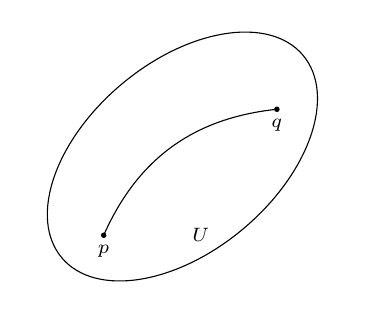
\begin{tikzpicture}
    \draw[rotate=40](0,0)ellipse(2 and 1.2);
    \path (-1, -1) edge [bend left] (1.2,0.6);
    \fill(1.2,0.6)circle(1pt)node[below]{\scriptsize\( q \)};
    \fill(-1, -1)circle(1pt)node[below]{\scriptsize\( p \)};
    %\draw[-latex,thick](-0.2,0.07)--(0.7,0.8)node[left,xshift=-0.1cm]{\scriptsize\( X \)};
    \node at(0,-1)[right]{\scriptsize\( U \)};
\end{tikzpicture}
\end{marginfigure}

对于一个区域$ U $,如果其中任意两点$p,q$都能由该区域内的点组成的曲线连接起来,那么我们称其为\textbf{道路连通}的.特殊的,对于满足过区域内任意一点$ p $的任意闭曲线$ L $,均可以\textbf{连续}的收缩到$ p $点,我们称这样的区域$ U $为\textbf{单连通}的.即如图中$ U $是单连通的,$ V $不是单连通的.
\begin{marginfigure}
    \centering
    \caption{非单连通区域$V$,$L_1$可以连续收缩回$ p $,但是$L_2$不能}
\begin{tikzpicture}
    % 绘制外层区域V
    \draw (-0.4,0) ellipse (2 and 1.2);
    \node at(-0.4,-1)[right]{\scriptsize\( V \)};
    
    % 绘制L1
    \draw (0.1,0) ellipse (0.5 and 0.7);
    \node at (0.6, -0.8) {$L_1$};
    
    % 绘制L2并填充斜线
    \begin{scope}
        \clip (-1.5,0) ellipse (2cm and 1.5cm);
        \fill[pattern=north east lines] (-1.2,0) ellipse (0.6cm and 0.4cm);
    \end{scope}
    \draw (-1.2,0) ellipse (0.8cm and 0.6cm);
    \node at (-0.9, 0.9) {$L_2$};
    
    % 绘制点p
    \fill (-0.4, 0.1) circle (1pt);
    \node at (-0.4, -0.4) {$p$};
\end{tikzpicture}
\end{marginfigure}
\subsubsection{$O(3)$群的道路连通性}
回忆$O(3)$群为3维正交群,其群元行列式为$\pm1$,首先假设存在这样的一条曲线$\gamma\in O(3)$,我们令这条曲线分别连接行列式为$+1$的群元$E_+$和行列式为$-1$的群元$E_-$,曲线自然被要求为连续的,其多项式函数:行列式自然同样被要求为连续的,但实际上行列式并不连续,自然得出$O(3)$\textbf{不是道路连通的}.

\subsubsection{$SO(3)$群的道路连通性}
既然$O(3)$不是道路连通的,那么我们继续考虑其特殊情况$SO(3)$群的情况.在前面,我们多次得出$SO(3)$可以表征$ 3 $维空间内的旋转,这自然吸引我们去使用更加形象化的表述去讨论其道路连通性.

我们在前面使用欧拉角给出过$SO(3)$的群元表达式
$$g=g_z^\alpha g_x^\beta g_z^\gamma$$

\begin{marginfigure}
    \centering
    \caption{$SO(3)$表征为球面,其中,$ p $与$ q $连接的曲线$\gamma_1$可以连续收缩到同一点,对于$ m,p,q,n $的任意除$m,n$的两两组合都满足这一关系,但是对于$m,n$两点,由于其关于球心对称,$ m $移动要求$ n $也需要同样对称的移动,故其始终保持一个大圆,不能收缩到同一点}
    \begin{tikzpicture}
        \def\R{2} % 切面半径
        \def\AngleGamma{0.1} % 极点倾斜角
        \fill[ball color=white] (0,0) circle (\R); % 3D 效果的球
        \coordinate[mark coordinate] (m) at (0,\R);
        \coordinate[mark coordinate] (n) at (0,-\R);
        \coordinate[mark coordinate] (p) at (\R*0.5,0.7);
        \coordinate[mark coordinate] (q) at (-\R*0.58,-0.3);
        \draw[rotate=20] (0,0.2) ellipse (1.2 and 0.7);
        \node at (0.6, 0.7) {$\gamma_1$};
        \node at (-0.5, -0.8*\R) {$\gamma_2$};
        \DrawLongitude{\R}{45};
        \node[above=8pt] at (m) {$m$};
        \node[below=8pt] at (n) {$n$};
        \node[below=8pt] at (p) {$p$};
        \node[below=8pt] at (q) {$q$};
    \end{tikzpicture}
\end{marginfigure}
其群元可以与一个三维空间内的单位球面建立起一一对应关系.另外,需要强调,关于球心对称的点应当视为同一类转动,于是对于图示情况,上面的曲线可以分类为$\gamma_1,\gamma_2$两类,一类可以连续收缩到同一点,另一类不行.于是我们称$SO(3)$为\textbf{双连通的}.

由于$SO(3)$为双连通的,为了寻找一个性质更好的群从而满足需求,这样我们便引入了单连通群$SU(2)$群.
\subsubsection{单连通群$SU(2)$}
对于$SU(2)$的群元$U$,存在其表示
\begin{equation}
    U=\begin{pmatrix}a&b\\-b^*&a^*\end{pmatrix}
\end{equation}
其中$a,b\in\mathbb C,aa^*+bb^*=1$,并且令$a=x_0+ix_1,b=x_2+ix_3$,存在关系
\begin{equation}
    x_0^2+x_1^2+x_2^2+x_3^2=1
\end{equation}
于是我们发现,$SU(2)$的群元$U$对应于四维空间$\mathbb R^4$中的三维球面$\mathbb S^3$上的一点,于是对于$SU(2)$连通性的研究可以转到对于三维球面$\mathbb S^3$的研究. 

对于$\bb S^3$,我们首先确定$x_0$,并且注意到当$x_0=\pm1$时为特殊情况,故先讨论$x_0\ne\pm1$.
\marginnote[]{分别对四个变量给定$$\begin{aligned}&x_{0}=\cos\frac{\theta}{2}\quad(0<\theta<360°)\\&x_{1}=\sin\frac{\theta}{2}\cos\alpha\\&x_{2}=\sin\frac{\theta}{2}\cos\beta\\&x_{3}=\sin\frac{\theta}{2}\cos\gamma\end{aligned} $$}我们给出了关于转轴$\mb n=(\cos\alpha,\cos\beta,\cos\gamma)$,转角$\theta$的关系.当我们取遍所有$x_0\ne\pm1$的点时,我们发现取到的区域占满了一个半径为$ 2 $个单位长度的\textbf{球体},但是球心和球面没有被取到.

对于$x_0=+1$时,其他变量均为$ 0 $,对应于球心,相应的,$x_0=-1$时对应于球面.显然,对于一个这样的球体,其为\textbf{单连通的}.
\subsubsection{$SU(2)$群与$SO(3)$群的2-1同态}
\marginnote[]{对于\textbf{同态}和\textbf{同构},如果两个群$G,G'$满足在映射$ f $下群乘法不变,即称$G,G'$是同态的,如果同态的同时还满足k-1映射,则称其为k-1同态.特别的,对于一一映射的情况,我们称$G,G'$是\textbf{同构}的.}
我们提到过,$SU(2)$是由于$SO(3)$群被引入的,在这一部分,我们将讨论二者之间的关联.

在量子力学中的学习,我们认识了\textbf{泡利矩阵},其相互正交,于是可以用来表示一个三维空间内的矢量$\mb{OP}=x\mb i+y\mb j+z\mb k$:
\begin{equation}
    P=x\sigma_x+y\sigma_y+z\sigma_z=\begin{pmatrix}z&x-\mathrm{i}y\\x+\mathrm{i}y&-z\end{pmatrix}
\end{equation}
显然$ P $是一个厄米矩阵,其迹为0\sidenote{回忆量子力学与线代知识,厄米矩阵即$U^\dagger=U$,求迹$\tr U$即主对角线求和.}.\\
取$SU(2)$的群元$Q$,对矩阵$ P $利用$ Q $构造相似矩阵$P'=QPQ^\dagger$,其可以表示为
\begin{equation}
    QPQ^\dagger=P^{\prime}=\begin{pmatrix}z^{\prime}&x^{\prime}-iy^{\prime}\\x^{\prime}+iy^{\prime}&-z^{\prime}\end{pmatrix}
\end{equation}
我们发现对于$x,y,z$与$x',y',z'$存在一个旋转矩阵$ R(\mb Q) $的变换,即在$SU(2)$和$O(3)$间建立了映射关系
\begin{marginfigure}
    \centering
    \caption{对应映射关系}
    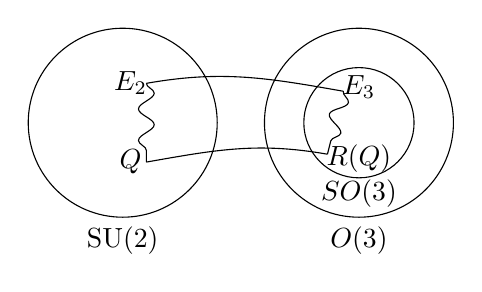
\begin{tikzpicture}
        \draw (0,0) ellipse (1.2cm and 1.2cm);
        \node at (0, -1.5) {SU(2)};
        \node at (0.1,0.5) {$E_2$};
        \node at (0.1,-0.5) {$\mb Q$};
        \draw (3,0) ellipse (1.2cm and 1.2cm);
        \node at (3, -1.5) {$O(3)$};
        \draw (3,0) ellipse (0.7cm and 0.7cm);
        \node at (3,-0.9) {$SO(3)$};
        
        \node at (3,0.45) {$E_3$};
        \node at (3,-0.45) {$R(\mb Q)$};
        \draw[-] (0.3,0.5) to [out=10,in=170] (2.8,0.4);
        \draw[-] (0.3,-0.5) to [out=10,in=170] (2.6,-0.4);
        \draw[decorate, decoration={snake, amplitude=1mm, segment length=4mm}] (0.3,0.5) -- (0.3,-0.5);
        \draw[decorate, decoration={snake, amplitude=1mm, segment length=4mm}] (2.8,0.4) -- (2.6,-0.4);
    \end{tikzpicture}
\end{marginfigure}
\begin{equation}
    \Map{R}{SU(2)}{O(3)}{\mb Q}{R(\mb Q)}
\end{equation}
考虑$\mb Q\maparrow R(\mb Q)$是连续的,且$SU(2)$是单连通群,于是$|R(\mb Q)|$是对于$\mb Q$的连续函数,并且对于幺元$|R(I_2)|=|I_3|=1$.因此,对于任意的$\mb Q\in SU(2)$,就有$R(\mb Q)\in SO(3)$

我们不加以证明的给出,单连通群$SU(2)$是双连通群$SO(3)$的一个\textbf{覆盖群}.这导致了费米子的半整数自旋,以及我们可以使用旋量表示电子.


\subsection{氢原子的$SO(4)$对称性}
虽然这一章侧重于数学内容的快速概览,但是适当结合一下物理应用是有益的,至少不会纠结这些东西究竟有什么用处.关于量子力学部分将会不再次介绍,默认读者已经了解这部分内容.

给定氢原子哈密顿量:$\displaystyle\hat{H}=\frac{\hat{\bm{p}^2}}{2\mu}-\frac{e^2}{r}$定义LRL矢量(拉普拉斯-龙格-楞次矢量,Laplace-Runge-Lenz矢量):
\begin{equation}
    \displaystyle \hat{\bm{A}}=\frac{1}{2\mu e^2}(\hat{\bm{p}}\times\hat{\bm{L}}-\hat{\bm{L}}\times\hat{\bm{p}})-\frac{\hat{\bm{r}}}{r}
\end{equation}
由对易关系$\displaystyle[\hat{L}_i,\hat{p}_j]=i\hbar \epsilon _{ijk}\hat{p}_k$,\sidenote{其中$\epsilon _{ijk}$为列维西维塔符号}将LRL矢量的分量写为
\begin{equation}
    \displaystyle\hat{A}_i=\frac{1}{2\mu e^2}\epsilon _{ijk}(\hat{p}_j\hat{L}_k-  \hat{L}_j\hat{p}_k)-\hat{n}_i   =\frac{1}{\mu e^2}\epsilon _{ijk}\hat{p}_j\hat{L}_k -\frac{i\hbar }{\mu e^2}\hat{p}_i-\hat{n}_i
\end{equation}
其中,$\displaystyle\hat{n}_i=\frac{\hat{r}_i}{r}$,相应有对易关系$[\hat{L}_i,\hat{n}_j  ]=i\hbar \epsilon _{ijk}\hat{n}_k $.计算LRL矢量的平方:
\begin{equation}
    \displaystyle\hat{\bm{A}^2}=\hat{A}_i \hat{A}_i =(\frac{1}{\mu e^2}\epsilon _{ijk}\hat{p}_j\hat{L}_k -\frac{i\hbar }{\mu e^2}\hat{p}_i-\hat{n}_i)(\frac{1}{\mu e^2}\epsilon _{ilm}\hat{p}_l\hat{L}_m -\frac{i\hbar }{\mu e^2}\hat{p}_i-\hat{n}_i)=\sum_{a=1}^{9}\hat{\Omega }  _a
\end{equation}

将括号展开得到$ 9 $项,形式比较复杂,需要熟悉掌握列维西维塔符号的使用,对于这个符号的介绍,请参考附录的内容.

分别计算,得出最终结果
\marginnote[]{
    利用了中心势场中$\hat{L}_k\hat{p}_k=\bm{\hat{L}}\cdot \bm{\hat{p}}=0$
$$\begin{align}\hat{\Omega }_1 &= \frac{1}{\mu ^2e^4}\epsilon _{ijk} \epsilon _{ilm}\hat{p}_j\hat{L}_k\hat{p}_l\hat{L}_m\\&=\frac{1}{\mu ^2e^4}(\delta _{jl}\delta _{km}-\delta _{jm}\delta _{kl})\hat{p}_j\hat{L}_k\hat{p}_l\hat{L}_m\\&= \frac{1}{\mu ^2e^4}(\hat{p}_j\hat{L}_k\hat{p}_j\hat{L}_k-\hat{p}_j \hat{L}_k\hat{p}_k \hat{L}_j)\\&=\frac{1}{\mu ^2e^4}\hat{p}_j\hat{L}_k\hat{p}_j\hat{L}_k\\&=\frac{1}{\mu ^2e^2}\hat{p}_j (i\hbar \epsilon _{kjl}\hat{p}_l+\hat{p}_j\hat{L}_k)\hat{L}_k\\&=\frac{1}{\mu ^2e^4}\hat{\bm{p}}^2\hat{\bm{L}} ^2    \end {align} $$
$$\begin{align}\hat{\Omega }_2 &=-\frac{i\hbar }{\mu ^2e^4}\epsilon _{ijk}\hat{p}_j\hat{L}_k\hat{p}_i \\& = -\frac{i\hbar }{\mu ^2e^4}\epsilon _{ijk}\hat{p}_j(i\hbar \hat{p}_m+\hat{p}_i \hat{L}_k  )\\&=\frac{\hbar ^2}{\mu ^2e^4}\epsilon _{ijk}\epsilon _{imk} \hat{p}_j\hat{p}_m-\frac{i\hbar }{\mu ^2e^4}\epsilon _{ijk}\hat{p}_j\hat{p}_i\hat{L}_k \\& =\frac{\hbar ^2}{\mu ^2e^4}(3\delta _{jm}- \delta _{jk}\delta _{mk}) \hat{p}_j\hat{p}_m\\& =\frac{2\hbar ^2}{\mu ^2e^4}\hat{\bm{p}}^2        \end {align} $$
$$\begin{align}\hat{\Omega }_3 &=-\frac{1}{\mu e^2}\epsilon _{ijk}\hat{p}_j\hat{L}_k\hat{n}_i\\& =-\frac{1}{\mu e^2}\epsilon _{ijk}\hat{p}_j(i\hbar \epsilon _{kim}\hat{n}_m+ \hat{n}_i\hat{L}_k) \\& =-\frac{i\hbar }{\mu e^2}\epsilon _{ijk}\epsilon _{kim} \hat{p}_j \hat{n}_m-\frac{1}{\mu e^2} \hat{p}_j\hat{n}_i\hat{L}_k\\& = -\frac{2i\hbar}{\mu e^2} \hat{p}_i\hat{n}_i-\frac{1}{\mu e^2} \frac{\hat{L}_k \hat{L}_k}{r}\\& =-\frac{2i\hbar}{\mu e^2}\hat{\bm{p}}\cdot  \hat{\bm{n}}-\frac{1}{\mu e^2}\frac{\hat{\bm{L}}^2}{r}     \end {align}$$
$$\begin{align}\hat{\Omega }_4 &=-\frac{i]\hbar }{\mu e^2}\epsilon _{ilm}\hat{p}_i\hat{p}_l\hat{L}_m=0      \end {align}$$
$$\begin{align}\hat{\Omega }_5=-\frac{\hbar ^2}{\mu'^2e^4}\hat{\bm{p}}^2        \end {align}$$
$$\begin{align}\hat{\Omega }_6=\frac{i\hbar }{\mu e^2}\hat{\bm{p}}\cdot  \hat{\bm{n}}         \end {align} $$
     这里利用了对易子$ \displaystyle[\hat{n}_i,\hat{p}_i]=i\hbar \frac{\partial }{\partial x_i}(\frac{x_i}{r} )=i\hbar \frac{2}{r}$
$$\begin{align}\hat{\Omega }_7&=\frac{i\hbar }{\mu e^2}\hat{n}_i\hat{p}_i  \\& =     \frac{i\hbar }{\mu e^2}([\hat{n}_i,\hat{p}_i]+\hat{p}_i\hat{n}_i)\\& =- \frac{\hbar^2 }{\mu e^2}\frac{2}{r} + \frac{i\hbar }{\mu e^2}\hat{p}_i\hat{n}_i\\& =- \frac{\hbar^2 }{\mu e^2}\frac{2}{r} + \frac{i\hbar }{\mu e^2}\hat{\bm{p}}\cdot \hat{\bm{n}}    \end {align} $$
$$\begin{align}\hat{\Omega }_8 &=-\frac{1}{\mu e^2}\epsilon _{ilm}\hat{n}_i\hat{p}_l\hat{L}_m \\& =-\frac{1}{\mu e^2}\frac{\hat{\bm{L}}^2 }{r}     \end {align} $$
$$\begin{align}\hat{\Omega }_9=\hat{n}_i \hat{n}_i=\bm{I}    \end {align} $$
    }
\begin{equation}
    \begin{align}\displaystyle \hat{\bm{A}^2} &=\sum_{a=1}^{9}\hat{\Omega }  _a \\& =\frac{1}{\mu ^2e^4}\hat{\bm{p}}^2\hat{\bm{L}}^2+\frac{\hbar ^2}{\mu ^2e^4}\hat{\bm{p}}^2-\frac{2}{\mu e^2}\frac{\hat{\bm{L}}^2}{r} - \frac{\hbar^2 }{\mu e^2}\frac{2}{r} +\bm{I} \\& =\frac{2}{\mu e^4}(\frac{\hat{\bm{p}}^2}{2\mu } \hat{\bm{L}}^2+\hbar ^2 \frac{\hat{\bm{p}}^2}{2\mu } - \frac{e^2}{r}\hat{\bm{L}}^2-\frac{e^2}{r}\hbar ^2 )+\bm{I} \\& =\frac{2}{\mu e^4}\hat{H}(\hat{\bm{L}}^2+\hbar ^2)+\bm{I} \end {align} 
\end{equation}
对于束缚态情况,$E<0$,将哈密顿量算符替换为$E$
\begin{equation}
    \displaystyle \hat{\bm{A}^2}=\frac{2E}{\mu e^4}(\hat{\bm{L}}^2+\hbar ^2)+\bm{I} 
\end{equation}
等价写为
\begin{equation}
    \displaystyle-\frac{\mu e^4}{2E}=- \frac{\mu e^4}{2E}\hat{\bm{A}}^2+ \hat{\bm{L}}^2+\hbar ^2=\hat{\bm{M}}^2+\hat{\bm{L}}^2+\hbar ^2
\end{equation}
其中,$\hat{\bm{M}} $是约化LRL矢量算符,定义为$\displaystyle\hat{\bm{M}}=\sqrt[]{-\frac{\mu e^4}{2E} }  \hat{\bm{A}}$,并且LRL矢量各分量对易关系为$\displaystyle[\hat{A}_i,\hat{A}_j ]=i\hbar (-\frac{2\hat{H} }{\mu e^4} )\epsilon _{ijk}\hat{L}_k $

于是得出
\begin{equation}
    \displaystyle[\hat{M}_i,\hat{M}_j ]=i\hbar \epsilon _{ijk}\hat{L}_k =[\hat{L}_i,\hat{L}_j]
\end{equation}
这样我们可以引入两个新的厄米算符把二者联系起来:$\displaystyle\hat{\bm{J}}_\pm =\frac{1}{2}(\hat{\bm{M}}\pm \hat{\bm{L}} )  $,验证其满足对易关系$[\hat{J}_{\pm i}, \hat{J}_{\pm j}]=i\hbar \epsilon _{ijk} \hat{J}_{\pm k};[\hat{J}_{+ i}, \hat{J}_{- j}]=0$.

我们称其为角动量算符,存在关系
\begin{equation}
    \displaystyle\hat{\bm{J}}^2_{+}= \hat{\bm{J}}^2_{-}=\frac{1}{4}(\hat{\bm{M}}^2+\hat{\bm{L}}^2) \pm \frac{1}{4}(\hat{\bm{M}}\cdot\hat{\bm{L}}+\hat{\bm{L}}\cdot \hat{\bm{M}}) 
\end{equation}
进而得出
\begin{equation}
    \displaystyle\hat{\bm{J}}^2_{+}= \hat{\bm{J}}^2_{-}=\frac{1}{4}(\hat{\bm{M}}^2+\hat{\bm{L}}^2) \qquad  \hat{\bm{M}}\cdot\hat{\bm{L}}+\hat{\bm{L}}\cdot \hat{\bm{M}}=0
\end{equation}
所以得到最后这个重要的结果
\begin{equation}
    \displaystyle-\frac{\mu e^4}{2E}=4\hat{\bm{J}}^2_++\hbar ^2  
\end{equation}
对于$\hat{\bm{J}}^2_+$的本征值,有
\begin{equation}
    \displaystyle\hat{\bm{J}}^2_+=j(j+1)\hbar^2 \qquad j=0,\frac{1}{2},1,\frac{3}{2},2,...
\end{equation}
氢原子中处于束缚态的电子具有的能级$ E $满足的代数方程为
\begin{equation}
    \begin{align}-\frac{\mu e^4}{2E(j)} &=4j(j+1)\hbar^2+\hbar ^2  \\&  =(4j^2+4j+1)\hbar^2\\& =(2j+1)^2\hbar^2\end{align}
\end{equation}
得到
$$\displaystyle E(j)=-\frac{\mu e^4}{\hbar^2}\frac{1}{2(2j+1)^2}\qquad j=0,\frac{1}{2},1,\frac{3}{2},2,...$$
即氢原子能级公式
\begin{equation}
    \displaystyle E_n=-\frac{\mu e^4}{\hbar^2}\frac{1}{2n^2}\qquad n=1,2,3,...
\end{equation}
对于$\hat{\bm{J}}_+$和$\hat{\bm{J}}_-$,回忆之前的李代数内容,不难发现其分别构成了$\mf{so}(3)$李代数,整体构成了$\mf{so}(4)=\mf{so}(3)\otimes\mf{so}(3)$李代数,即$SO(4)$对称性的来源,我们发现这种方法仅可以得到本征值,不能得到径向波函数的特征.
\subsection{再论氢原子: $\mf{so}(2,1)$李代数}
1




\section{流形与流形上的外微分}
\subsection{流形}
1
\section{纤维丛}
\subsection{切丛与余切丛}
1
\section{辛几何与辛结构}
\subsection{辛形式和辛流形}
1
\section{同调群}
\subsection{单纯复合形}
1
\section{De Rham 上同调群}
\subsection{流形上的De Rham 上同调群}
1
\section{仿射联络空间与黎曼流形}
\subsection{仿射联络}
1















